\documentclass[
	% -- opções da classe memoir --
	12pt,				% tamanho da fonte
	%openright,			% capítulos começam em pág ímpar (insere página vazia caso preciso)
	%twoside,			% para impressão em recto e verso. Oposto a oneside
	oneside,
	a4paper,			% tamanho do papel. 
	% -- opções da classe abntex2 --
	%chapter=TITLE,		% títulos de capítulos convertidos em letras maiúsculas
	%section=TITLE,		% títulos de seções convertidos em letras maiúsculas
	%subsection=TITLE,	% títulos de subseções convertidos em letras maiúsculas
	%subsubsection=TITLE,% títulos de subsubseções convertidos em letras maiúsculas
	% -- opções do pacote babel --
	english,			% idioma adicional para hifenização
	german,				% idioma adicional para hifenização
	brazil				% o último idioma é o principal do documento
	]{abntex2}

% ---
% Pacotes básicos 
% ---
\usepackage{float}
\usepackage{lmodern}			% Usa a fonte Latin Modern			
\usepackage[T1]{fontenc}		% Selecao de codigos de fonte.
\usepackage[utf8]{inputenc}		% Codificação do documento (conversão automática dos acentos)
\usepackage{lastpage}			% Usado pela Ficha catalográfica
\usepackage{indentfirst}		% Indenta o primeiro parágrafo de cada seção.
\usepackage{color}				% Controle das cores
\usepackage{graphicx}			% Inclusão de gráficos 
\usepackage{svg}
\usepackage{microtype} 			% para melhorias de justificação
\usepackage{amsmath}
\usepackage{amssymb}
\usepackage{physics}
\usepackage{mathtools}
\usepackage{xfrac}
% ---
		
% ---
% Pacotes adicionais, usados apenas no âmbito do Modelo Canônico do abnteX2
% ---
\usepackage{lipsum}				% para geração de dummy text
% ---

% ---
% Pacotes de citações
% ---
\usepackage[brazilian,hyperpageref]{backref}	 % Paginas com as citações na bibl
\usepackage[alf]{abntex2cite}	% Citações padrão ABNT

% --- 
% CONFIGURAÇÕES DE PACOTES
% --- 

% ---
% Configurações do pacote backref
% Usado sem a opção hyperpageref de backref
\renewcommand{\backrefpagesname}{Citado na(s) página(s):~}
% Texto padrão antes do número das páginas
\renewcommand{\backref}{}
% Define os textos da citação
\renewcommand*{\backrefalt}[4]{
	\ifcase #1 %
		Nenhuma citação no texto.%
	\or
		Citado na página #2.%
	\else
		Citado #1 vezes nas páginas #2.%
	\fi}%
% ---


\usepackage[portuguese, onelanguage, ruled, vlined]{algorithm2e}
%\usepackage{algpseudocode}


% ---
% Informações de dados para CAPA e FOLHA DE ROSTO
% ---
\titulo{Seleção Incremental de Variáveis para Aprendizado de
Máquina utilizando Preditor Linear e Validação Cruzada}
\autor{João Victor Barbosa Alves}
\local{Belo Horizonte, Minas Gerais - Brasil}
\data{2018}
\orientador{Antônio de Pádua Braga}
\instituicao{%
  Universidade Federal de Minas Gerais - UFMG
  \par
  Escola de Engenharia
  \par
  Programa de Graduação em Engenharia Elétrica}
\tipotrabalho{Trabalho de conclusão de curso - TCC}
% O preambulo deve conter o tipo do trabalho, o objetivo, 
% o nome da instituição e a área de concentração 
\preambulo{Lorem ipsum dolor sit amet, consectetur adipiscing elit. Phasellus lacinia, erat vitae pulvinar malesuada, dolor enim laoreet lectus, a tincidunt lorem lorem in lorem. Suspendisse sagittis sem ex.}
% ---


% ---
% Configurações de aparência do PDF final

% alterando o aspecto da cor azul
\definecolor{blue}{RGB}{41,5,195}

% informações do PDF
\makeatletter
\hypersetup{
     	%pagebackref=true,
		pdftitle={\@title}, 
		pdfauthor={\@author},
    	pdfsubject={\imprimirpreambulo},
	    pdfcreator={LaTeX with abnTeX2},
		pdfkeywords={abnt}{latex}{abntex}{abntex2}{trabalho acadêmico}, 
		colorlinks=true,       		% false: boxed links; true: colored links
    	linkcolor=blue,          	% color of internal links
    	citecolor=blue,        		% color of links to bibliography
    	filecolor=magenta,      		% color of file links
		urlcolor=blue,
		bookmarksdepth=4
}
\makeatother
% --- 

% --- 
% Espaçamentos entre linhas e parágrafos 
% --- 

% O tamanho do parágrafo é dado por:
\setlength{\parindent}{1.3cm}

% Controle do espaçamento entre um parágrafo e outro:
\setlength{\parskip}{0.2cm}  % tente também \onelineskip


% ---
% compila o indice
% ---
\makeindex
% ---

% ----
% Início do documento
% ----
\begin{document}

% Seleciona o idioma do documento (conforme pacotes do babel)
%\selectlanguage{english}
\selectlanguage{brazil}

% Retira espaço extra obsoleto entre as frases.
\frenchspacing 

% ----------------------------------------------------------
% ELEMENTOS PRÉ-TEXTUAIS
% ----------------------------------------------------------
% \pretextual

% ---
% Capa
% ---
\imprimircapa
% ---

% ---
% Folha de rosto
% (o * indica que haverá a ficha bibliográfica)
% ---
\imprimirfolhaderosto*
% ---

% ---
% Inserir a ficha bibliografica
% ---

% ---


% ---
% Inserir folha de aprovação
% ---

% Isto é um exemplo de Folha de aprovação, elemento obrigatório da NBR
% 14724/2011 (seção 4.2.1.3). Você pode utilizar este modelo até a aprovação
% do trabalho. Após isso, substitua todo o conteúdo deste arquivo por uma
% imagem da página assinada pela banca com o comando abaixo:
%
% \includepdf{folhadeaprovacao_final.pdf}
%
\begin{folhadeaprovacao}

  \begin{center}
    {\ABNTEXchapterfont\large\imprimirautor}

    \vspace*{\fill}\vspace*{\fill}
    \begin{center}
      \ABNTEXchapterfont\bfseries\Large\imprimirtitulo
    \end{center}
    \vspace*{\fill}
    
    \hspace{.45\textwidth}
    \begin{minipage}{.5\textwidth}
        \imprimirpreambulo
    \end{minipage}%
    \vspace*{\fill}
   \end{center}
        
   \centering 
   Trabalho aprovado. \today:

   \assinatura{\textbf{\imprimirorientador} \\ Orientador} 
   \assinatura{\textbf{Professor} \\ Convidado 1}
   \assinatura{\textbf{Professor} \\ Convidado 2}
   %\assinatura{\textbf{Professor} \\ Convidado 3}
   %\assinatura{\textbf{Professor} \\ Convidado 4}
      
   \begin{center}
    \vspace*{0.5cm}
    {\large\imprimirlocal}
    \par
    {\large\imprimirdata}
    \vspace*{1cm}
  \end{center}
  
\end{folhadeaprovacao}
% ---


% ---
% Agradecimentos
% ---
% \begin{agradecimentos}
% Os agradecimentos principais são direcionados à Gerald Weber, Miguel Frasson,
% Leslie H. Watter, Bruno Parente Lima, Flávio de Vasconcellos Corrêa, Otavio Real
% Salvador, Renato Machnievscz\footnote{Os nomes dos integrantes do primeiro
% projeto abn\TeX\ foram extraídos de
% \url{http://codigolivre.org.br/projects/abntex/}} e todos aqueles que
% contribuíram para que a produção de trabalhos acadêmicos conforme
% as normas ABNT com \LaTeX\ fosse possível.

% Agradecimentos especiais são direcionados ao Centro de Pesquisa em Arquitetura
% da Informação\footnote{\url{http://www.cpai.unb.br/}} da Universidade de
% Brasília (CPAI), ao grupo de usuários
% \emph{latex-br}\footnote{\url{http://groups.google.com/group/latex-br}} e aos
% novos voluntários do grupo
% \emph{\abnTeX}\footnote{\url{http://groups.google.com/group/abntex2} e
% \url{http://www.abntex.net.br/}}~que contribuíram e que ainda
% contribuirão para a evolução do \abnTeX.

% \end{agradecimentos}
% ---

% ---
% Epígrafe
% ---
\begin{epigrafe}
    \vspace*{\fill}
	\begin{flushright}
		\textit{São as perguntas que não sabemos responder que mais nos ensinam. \\
		Elas nos ensinam a pensar. \\
		Se você dá uma resposta a um homem, tudo o que ele ganha é um fato qualquer. \\
		Mas, se você lhe der uma pergunta, ele procurará suas próprias respostas. \\
		(…) \\
        Assim, quando ele encontrar as respostas, elas lhe serão preciosas. \\
        Quanto mais difícil a pergunta, com mais empenho procuramos a resposta. \\
        Quanto mais a procuramos, mais aprendemos. \\
        Rothfuss, Patrick - O Temor do Sábio - a Crônica do Matador do Rei - Segundo Dia.}
	\end{flushright}
\end{epigrafe}
% ---

% ---
% RESUMOS
% ---

% resumo em português
\setlength{\absparsep}{18pt} % ajusta o espaçamento dos parágrafos do resumo
\begin{resumo}
\lipsum[1]
 \textbf{Palavras-chave}: latex. abntex. editoração de texto.
\end{resumo}

% % resumo em inglês
% \begin{resumo}[Abstract]
%  \begin{otherlanguage*}{english}
%   This is the english abstract.

%   \vspace{\onelineskip}
 
%   \noindent 
%   \textbf{Keywords}: latex. abntex. text editoration.
%  \end{otherlanguage*}
% \end{resumo}

% ---
% inserir lista de ilustrações
% ---
% \pdfbookmark[0]{\listfigurename}{lof}
% \listoffigures*
% \cleardoublepage
% ---

% ---
% inserir lista de tabelas
% ---
% \pdfbookmark[0]{\listtablename}{lot}
% \listoftables*
% \cleardoublepage
% ---

% ---
% inserir lista de abreviaturas e siglas
% % ---
% \begin{siglas}
%   \item[ABNT] Associação Brasileira de Normas Técnicas
%   \item[abnTeX] ABsurdas Normas para TeX
% \end{siglas}
% % ---

% ---
% inserir lista de símbolos
% ---
% \begin{simbolos}
%   \item[$ \Gamma $] Letra grega Gama
%   \item[$ \Lambda $] Lambda
%   \item[$ \zeta $] Letra grega minúscula zeta
%   \item[$ \in $] Pertence
% \end{simbolos}
% ---

% ---
% inserir o sumario
% ---
\pdfbookmark[0]{\contentsname}{toc}
\tableofcontents*
\cleardoublepage
% ---



% ----------------------------------------------------------
% ELEMENTOS TEXTUAIS
% ----------------------------------------------------------
\textual

\chapter[Introdução]{Introdução}

O aumento da capacidade de armazenamento e processamento de dados tem possibilitado o desenvolvimento de sistemas inteligentes através do aprendizado de máquina. Tal desenvolvimento, por sua vez, permitiu avanços em diversas áreas da computação, microeletrônica e sensoriamento. 

Hoje, aplicações tais como pesquisas web, sistemas \textit{anti-spam}, reconhecimento de voz, recomendações de produto e diversas outras são frutos desse progresso. Porém a disponibilidade de quantidades massivas de dados, apresenta não só um horizonte vasto de possíveis aplicações, mas também desafios para seleção e processamento desses dados.


\section{Aprendizado de Máquina}

Aprendizado de máquina é o campo da computação responsável por desenvolver e empregar sistemas ou modelos que, através da sua exposição à experiências, são capazes de melhorar sua performance na realização de determinada tarefa \cite{mitchell_1997}.

O processo de desenvolvimento de modelos com aprendizado de máquina pode ser dividido, em linhas gerais, em duas grandes etapas. 

Inicialmente os dados disponíveis são analisados e tratados. Nessa etapa procura-se identificar correlações entre as informações disponíveis e as variáveis de interesse. Além disso, são explorados possíveis filtros, transformações e outros algoritmos que possam facilitar o aprendizado do modelo. Também é necessário realizar nessa etapa a separação dos dos dados que serão utilizados para treinamento, validação e teste no decorrer do processo.

Na etapa seguinte objetiva-se obter um modelo capaz de reproduzir o comportamento do sistema que gerou o conjunto de dados. Para tal, um ou mais modelos e algoritmos são selecionados e o treinamento é realizado. Duas características são de fundamental importância e devem ser controladas: a capacidade de assimilação do comportamento representado pelos dados (complexidade) e a capacidade de extrapolação das saídas para novas entradas (generalização).


\begin{figure}[H]
    \caption{\textcolor{red}{ADAPTAR:} Fluxo de desenvolvimento de sistemas inteligentes. }
    \begin{center}
    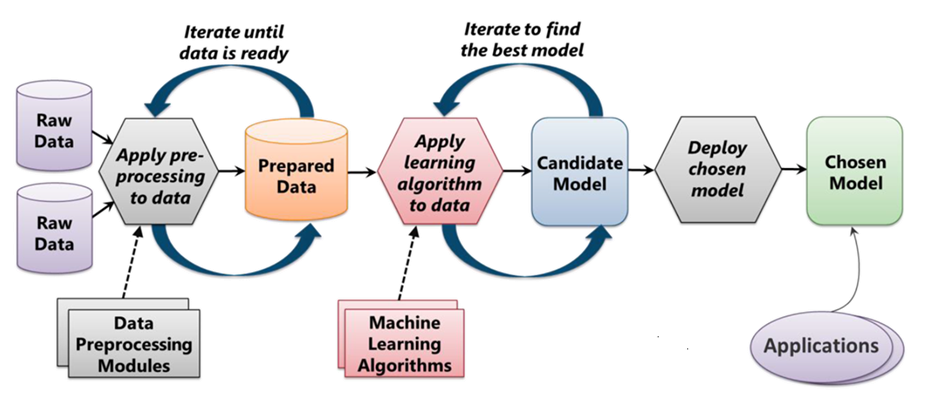
\includegraphics[width=\linewidth]{imgs/intro/MLFlow.png}
    \end{center}
    \legend{Fonte: \textit{Introduction to Microsoft Azure by David Chappell}.}
    \label{fig:mlflow}
\end{figure}

Os algoritmos utilizados nesta segunda etapa podem ser classificados em uma de três categorias, de acordo com as características dos dados disponíveis. \cite{ai_modern}

Na categoria de aprendizado não supervisionado, desenvolve-se sistemas capazes identificar padrões implícitos em um conjunto de dados não rotulados.

No aprendizado por reforço, os sistemas se adaptam de acordo com dados de resposta oriundos do ambiente no qual estão envolvidos.

Por fim, no aprendizado supervisionado, estão modelos que, a partir de um conjunto de entradas e saídas conhecidas, são capazes de extrapolar a dinâmica do sistema em questão.


\section{Generalização}

Generalização é o termo usado para descrever a capacidade de um sistema de reagir a novos dados. Isto é, após realizado o treinamento, a capacidade de um sistema de realizar predições precisas para dados nunca observados.

O processo de aprendizado supervisionado é a inferência de um mapeamento de dados de entrada a variáveis de saída a partir de um conjunto de observações. Este pode, portanto, ser interpretado como um ajuste não linear de uma curva \cite{haykin}. Consequentemente, os modelos obtidos através desse processo também estão sujeitos a \textit{overfitting} e \textit{underfitting}.

\textit{Overfitting}, ou sobre-ajuste, é caracterizado pela alta performance no conjunto de dados de treinamento e baixa performance em dados nunca observados. Isto é, o modelo assimila desvios causados por erros de medição ou fatores aleatórios presentes no treinamento. Dessa maneira, o erro em relação aos dados de treinamento é reduzido, porém essa melhora não corresponde a uma melhora na representação da realidade.

De maneira similar, o \textit{underfitting},ou sub-ajuste, é caracterizado pela baixa performance em ambos os conjuntos de dados, indicando que o modelo utilizado não é capaz de representar de maneira satisfatória a complexidade do sistema real.

\begin{figure}[H]
    \caption{Exemplo de underfitting, ajuste ideal e overfitting.}
    \begin{center}
    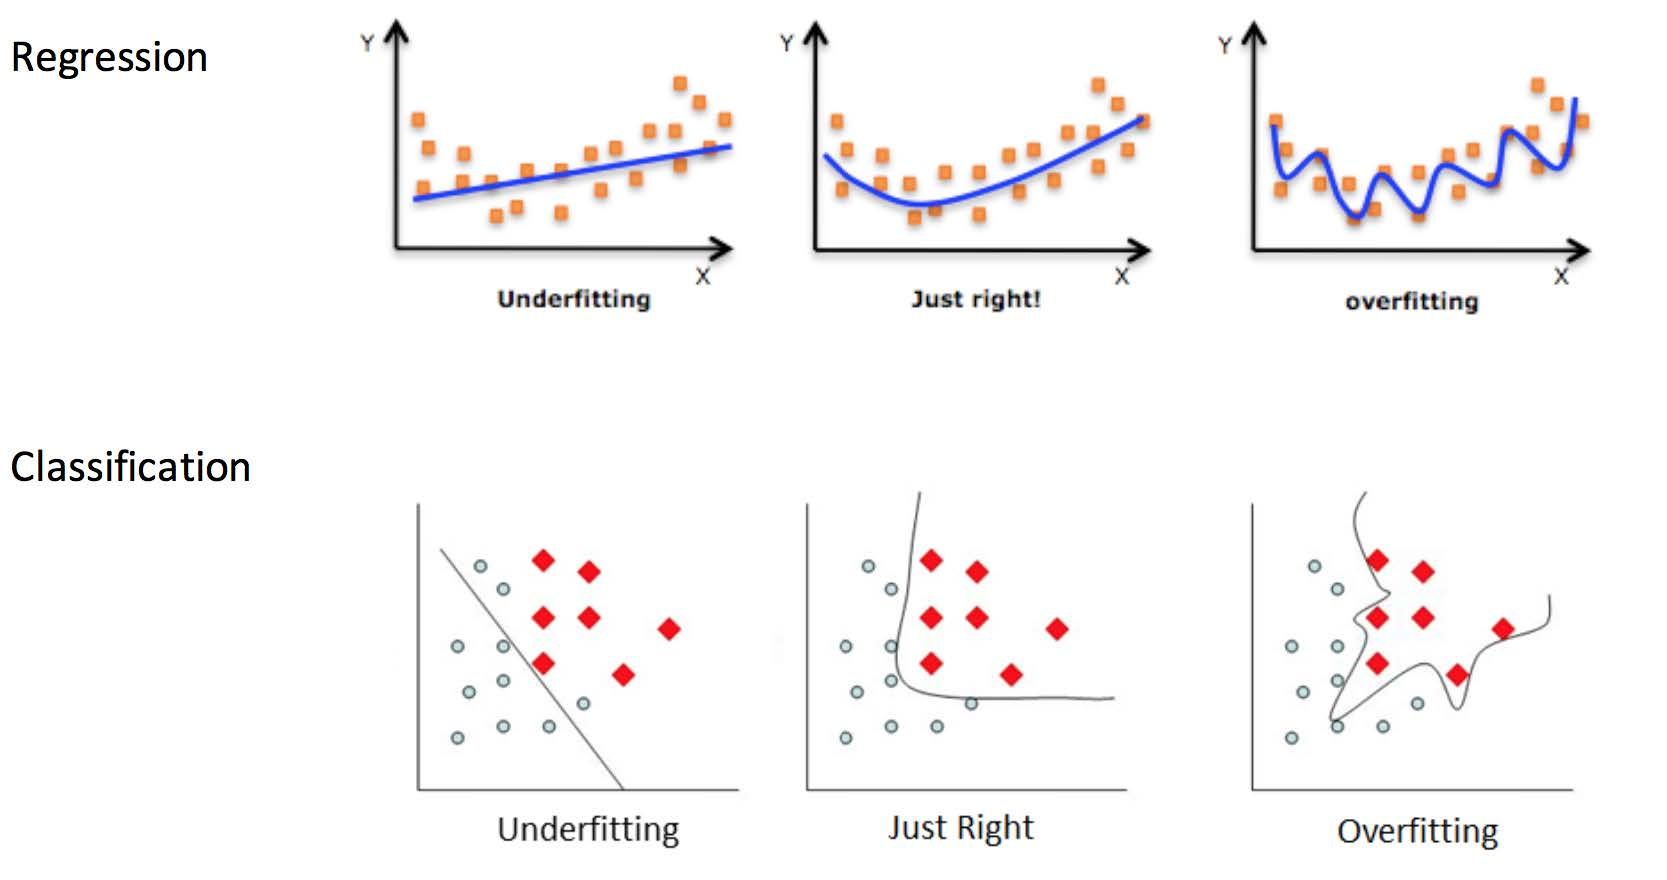
\includegraphics[width=\linewidth]{imgs/intro/overfit}
    \end{center}
    \legend{Fonte: }
    \label{fig:mlflow}
\end{figure}


Enquanto a escolha de um modelo adequado é suficiente para evitar o \textit{underfitting}, diversos fatores contribuem podem contribuir para a ocorrência de \textit{overfitting}. 

\section{Objetivos}

Esse trabalho apresenta um método de seleção de variáveis de entrada para modelos treinados através de aprendizado supervisionado. 

O algoritmo a ser descrito estima o desempenho das variáveis individualmente e em conjunto através do treinamento de modelos lineares e do cálculo de sua performance aplicando a estratégia de validação cruzada.
\chapter[Fundamentação Teórica]{Fundamentação Teórica}

Nesta seção são abordados conceitos fundamentais para a compreensão deste trabalho, assim como tendências atuais da literatura em relação ao tema estudado.

\section{Regressão Linear}

Os modelos de regressão linear constituem uma classe de modelos que utilizam funções lineares com parâmetros ajustáveis. O exemplo mais simples dessa classe é a função que realiza a combinação linear das entradas com os parâmetros ajustados para gerar uma predição (eq. \ref{eq:lin_expandida}).

\begin{equation}
    \hat{y} = w_0 + w_1x_1+ ... + w_px_p = \sum_{i = 0}^{p} w_iX = XW
    \label{eq:lin_expandida}
\end{equation}

Onde $p$ corresponde ao número de dimensões da variável de entrada e $x_0 = 1$.

Modelos mais complexos e de maior aplicabilidade podem ser obtidos ao se considerar um conjunto fixo de 
transformações não-lineares ($\phi_n(X)$) ao invés das variáveis originais, ou em conjunto com elas. 
Esses modelos são lineares em relação as suas variáveis independentes, porém são não-lineares em relação 
as variáveis de entrada \cite{bishop_2006}.

\subsection{Treinamento de modelos lineares}

O treinamento de modelos lineares consiste em encontrar o vetor de parâmetros $W$ que maximize a similaridade entre o modelo e sistema modelado. Esse treinamento é normalmente realizado minimizando-se o somatório dos erros quadráticos (eq. \ref{eq:sq_error}) em função do vetor $W$.

% \begin{align}
% \begin{split}
%       E_{sq}(W) {}&= \frac{1}{2} \sum_{n = 1}^{N}\left(y_n-\hat{y}_n\right)^2 = \frac{1}{2} \sum_{n = 1}^{N} \left(y_n-\phi(X_n)W\right)^2
%     \label{eq:sq_error}  
% \end{split}\\
% \begin{split}
%     \pdv{E_{sq}(W)}{W} {}&= \sum_{n = 1}^{N} \phi(X_n)^T\left(\phi(X_n)W - y_n\right)
%     \label{eq:min_sq_error}
% \end{split}
% \end{align}

\begin{equation}
\begin{split}
      E_{sq}(W) {}&= \frac{1}{2} \sum_{n = 1}^{N}\left(y_n-\hat{y}_n\right)^2 \\
      &= \frac{1}{2} (Y-\hat{Y})^T(Y-\hat{Y})\\
      &= \frac{1}{2} \left( Y^TY - 2 \hat{Y}^TY + \hat{Y}^T\hat{Y} \right)\\
      &= \frac{1}{2} \left( Y^TY - 2 W^TX^TY + \sum_{n = 1}^{N}\left(X_nW \right)^2 \right)
    \label{eq:sq_error}  
\end{split}
\end{equation}

\begin{equation}\begin{split}
    \pdv{E_{sq}(W)}{W} &= \frac{1}{2} \left( 0 - 2 X^TY + 2\sum_{n = 1}^{N}\left(X_n^TX_n \right)W  \right) \\
    &= - X^TY + X^TX W
    \label{eq:min_sq_error}
\end{split}\end{equation}

Igualando-se a eq. \ref{eq:min_sq_error} a zero e isolando o vetor $W$, obtém-se a eq. \ref{eq:lsnormal}, conhecida como a equação normal para o problema dos mínimos quadrados.

\begin{equation}\begin{split}
    X^TX W &= X^TY \\
    W &= (X^TX)^{-1}X^TY \\
    W &=X^+ Y
    \label{eq:lsnormal}
\end{split}\end{equation}

O termo $(X^TX)$ pode se aproximar de uma matriz singular se muitas das variáveis envolvidas forem 
linearmente dependentes, resultando assim em dificuldades para o cálculo numérico dos valores e possivelmente em 
um vetor de parâmetros de alta magnitude. Um termo de regularização pode ser adicionado na eq. \ref{eq:sq_error} 
para minimizar esse problema, garantindo que a nova matriz não é singular.

A adição do termo de regularização tem ainda o efeito de limitar a complexidade efetiva do modelo, reduzindo o 
\textit{overfitting} e possibilitando a utilização de conjuntos de dados menores \cite{bishop_2006}.

Comumente utiliza-se norma-L2 do vetor de parâmetros como termo de regularização, dando origem a \textit{ridge 
regression}. A dedução da equação normal com termo de regularização é análoga à apresentada e resulta na eq. 
\ref{eq:lsnormal_reg}.

\begin{equation}\begin{split}
    W &= (\lambda I + X^TX)^{-1}X^TY = A^{-1}X_{[i]}^TY
    \label{eq:lsnormal_reg}
\end{split}\end{equation}



\section{Validação Cruzada}

A validação cruzada (\textit{cross-validation}) é um conjunto de metodologias de treinamento e validação que, de maneira simples e efetiva, permitem a estimativa do erro de generalização do modelo.

No método \textit{k-fold} de validação cruzada, os dados de treinamento são divididos em k conjuntos aleatórios de tamanhos aproximadamente iguais. Realizada essa divisão, a cada iteração do treinamento, os parâmetros do modelo são determinados utilizando k-1 conjuntos e sua performance é avaliada no conjunto restante. O processo se repete até que todos os k conjuntos tenham sido utilizados para avaliação e a média das performances observadas fornecem uma estimativa da performance de generalização do modelo \cite{overfitting_crossval}.

\begin{figure}[H]
    \centering
    \caption{Validação cruzada: \textit{5-fold}.}
    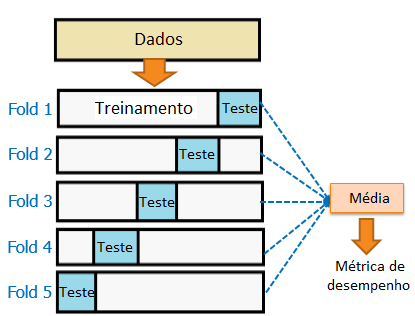
\includegraphics[width=0.7\textwidth]{imgs/rev/cross_validation}
    \legend{\textit{Fonte: Different types of Validations in Machine Learning (Cross Validation)} \cite{cross_val}}
    \label{fig:dim_perf}
\end{figure}

Um caso especial do método descrito é o \textit{leave-one-out cross-validation} (LOOCV), onde k é igual ao total de 
amostras disponíveis (N), ou seja, o treinamento é realizado N vezes com N-1 amostras, e validado na amostra excluída.
 Tal abordagem apesar de apresentar, em geral, um custo computacional elevado, resulta em um modelo com menor 
 variabilidade e viés para modelos de regressão linear \cite{burman}, produzindo assim resultados com melhor 
 performance e menos \textit{overfitting}.

\subsection{ \textit{Leave-one-out Cross-validation} e Regressão Linear}

Especificamente para o caso do preditor linear, é possível determinar o resultado do LOOCV sem a necessidade de se 
calcular N preditores, tornando essa uma estratégia interessante para determinar a capacidade de generalização de 
um modelo linear. A seguir uma dedução adaptada de \cite[p. 268]{lin_reg_analysis} é apresentada.

O erro de LOOCV corresponde a média dos erros quadráticos de cada estimador obtido excluindo-se uma amostra. 

\begin{equation}
    LOOCV = \dfrac{1}{N} \sum_{i=1}^{N}e^2_{[i]}
    \label{eq:cv_error}
\end{equation}
\begin{equation}
    e_{[i]} = y_i - \hat{y}_{[i]} = y_i - x_iW_{[i]} 
    \label{eq:ith_error}
\end{equation}
Onde o $i$ indexa a amostra excluída no treinamento, $\hat{y}_{[i]}$ corresponde à saída do preditor calculado sem a
amostra $(x_i,y_i)$ e $W_{[i]}$ os parâmetros desse preditor.

Pode-se definir o vetor de parâmetros $W_{[i]}$ conforme a eq. \ref{eq:wi}.
\begin{equation}
    W_{[i]} = A_{[i]}^{-1}X_{[i]}^TY_{[i]}
    \label{eq:wi}
\end{equation} 

É possivel perceber as seguintes igualdades:
\smallskip\noindent
\begin{equation}
    \begin{split}
        A_{[i]} &= \lambda I + X_{[i]}^TX_{[i]} \\
                &= \lambda I + X^TX - x_i^Tx_i \\
                &= A - x_i^Tx_i    
    \end{split}
    \label{eq:ai_identity}
\end{equation} 

\begin{equation}
    X_{[i]}^TY_{[i]} = X^TY - x_i^Ty_i
    \label{eq:X_iY_i_identity}
\end{equation} 

Aplicando a formula de Sherman–Morrison à eq. \ref{eq:ai_identity}, temos:
\smallskip\noindent
\begin{equation}
    \begin{split}        
       h_i &= x_iA^{-1}x_i^T \\
       A_{[i]}^{-1} &= A^{-1} + \dfrac{A^{-1}x_ix_i^TA^{-1}}{1-h_i}
    \end{split}
    \label{eq:sherman}
\end{equation}

Substituindo as eq. \ref{eq:X_iY_i_identity} e \ref{eq:sherman} na eq. \ref{eq:wi}.
\smallskip\noindent
\begin{equation}
    \begin{split}
        W_{[i]} &= \left(A^{-1} + \dfrac{A^{-1}x_i^Tx_iA^{-1}}{1-h_i}\right) \left(X^TY - x_i^Ty_i\right)\\
                &= W - A^{-1}x_i^Ty_i + \dfrac{A^{-1}x_i^Tx_iW}{1-h_i} - \dfrac{A^{-1}x_i^Tx_iA^{-1}x_i^Ty_i}{1-h_i} \\
                &= W - \dfrac{A^{-1}x_i^T}{1-h_i}\left(  y_i(1-h_i)-x_iW  + h_iy_i \right)  \\
                &= W - \dfrac{A^{-1}x_i^T}{1-h_i}\left(  y_i-\hat{y}_i \right)  \\
    \end{split}
    \label{eq:wi_expandido}
\end{equation}

Substituindo a eq. \ref{eq:wi_expandido} na eq. \ref{eq:ith_error}.
\smallskip\noindent
\begin{equation}
    \begin{split}
        e_{[i]} &= y_i - x_iW_{[i]} \\
                &= y_i - x_i\left( W - \dfrac{A^{-1}x_i^T}{1-h_i}\left(  y_i-\hat{y}_i \right) \right) \\
                &= y_i - \hat{y}_i + \dfrac{h_i}{1-h_i}\left(  y_i-\hat{y}_i \right) \\
                &= \dfrac{y_i- \hat{y}_i}{1-h_i}
    \end{split}    
    \label{eq:ith_error_expandido}
\end{equation}

Seja $P$ a matriz de projeção \cite[p. 303]{applied_matrix_algebra} do preditor (também conhecida como matriz chapéu
 \cite[p. 266]{lin_reg_analysis}) e a matriz de aniquilação $M$ \cite[p. 18]{econometrics} definidas conforme a eq. \ref{eq:proj_res_matrix}
\smallskip\noindent
\begin{equation}
    \begin{split}
        \hat{Y} &= PY \implies P = XA^{-1}X^T \\
        MY &= Y - \hat{Y} \implies M = I - P = I - XA^{-1}X^T
    \end{split}    
    \label{eq:proj_res_matrix}
\end{equation}

Para cada índice $i$, o numerador da eq. \ref{eq:ith_error_expandido} corresponde a linha de mesmo índice da matriz $MY$. 
Além disso o denominador da equação corresponde ao elemento da diagonal da matriz $M$ de mesmo índice. 
A partir dessas observações, pode-se agrupar todos os valores de $e_{[i]}$ na forma da matriz $E_{LOOCV}$, conforme a equação \ref{eq:e_cv}.
\smallskip\noindent
\begin{equation}
    \begin{split}
        E_{LOOCV} = diag(M)^{-1}MY
    \end{split}    
    \label{eq:e_cv}
\end{equation}

Como a matriz $M$ é simétrica, a eq. \ref{eq:cv_error} pode ser reescrita conforme eq. \ref{eq:LOOCV_error}.

\begin{equation}
    \begin{split}
        LOOCV   &= \dfrac{1}{N} \sum_{i=1}^{N}e^2_{[i]} \\
                &= \dfrac{1}{N} E_{LOOCV}^2 \\
                &= \dfrac{1}{N}E_{LOOCV}^TE_{LOOCV} \\
                &= \dfrac{1}{N} Y^TM\ diag(R)^{-2}MY \\
    \end{split}
    \label{eq:LOOCV_error}
\end{equation}


\section{Aprendizado Incremental}

A atualização dos parâmetros do modelo de regressão linear para uma nova amostra pode ser realizada de maneira 
incremental, sem a necessidade de se calcular um novo modelo \cite{mit_onlinereg}. Nesse trabalho porém, é de 
interesse calcular a atualização incremental ao se adicionar uma nova variável. Em especial, é de 
interesse a determinação de uma forma fechada para a matriz de aniquilação, usada no calculo do erro de 
validação cruzada.

A matrizes de interesse para o problema de dimensão $p+1$ tem a forma descrita na eq. \ref{eq:inc_matrix} 
\begin{equation}
    \begin{split}
    X_{p+1} &= \left[\mathbf{X_p}\ x_{p+1}\right] \\
    Y_{p+1} &= \left[\mathbf{Y_p}\ y_{p+1}\right] \\
    A_{p+1} &= (X_{p+1}^T X_{p+1} + \lambda I ) = 
    \begin{bmatrix}
        \mathbf{A_p} & \mathbf{X_p}^T x_{p+1} \\
        x_{p+1}^T \mathbf{X_p} & x_{p+1}^T x_{p+1} + \lambda
    \end{bmatrix}  \\
    M_{p+1} &= I - X_{p+1} A_{p+1}^{-1} X_{p+1}^T \\ 
    \end{split}  
    \label{eq:inc_matrix}
\end{equation}

É necessário então determinar a matriz $A_{p+1}^{-1}$ em função das matrizes já conhecidas. Para tal, aplica-se 
a identidade da inversa de uma matriz em blocos, conforme a eq. \ref{eq:blockinverse}, na matriz $A_{p+1}$.
\smallskip
\begin{equation}
    \begin{split}
        \Delta &= (\mathbf{D}-\mathbf{CA}^{-1}\mathbf{B}) \\
        \begin{bmatrix}
            \mathbf{A} & \mathbf{B} \\ 
            \mathbf{C} & \mathbf{D} 
        \end{bmatrix}^{-1} &= 
        \begin{bmatrix} 
            \mathbf{A}^{-1} & 0 \\ 
            0 & 0 
        \end{bmatrix} +        
        \begin{bmatrix} 
            \mathbf{A}^{-1}\mathbf{B}\Delta^{-1}\mathbf{CA}^{-1} & -\mathbf{A}^{-1}\mathbf{B}\Delta^{-1} \\ 
            -\Delta^{-1}\mathbf{CA}^{-1} & \Delta^{-1} 
        \end{bmatrix}
    \end{split}
    \label{eq:blockinverse}
\end{equation}

Através da eq. \ref{eq:inc_matrix}, obtém-se os termos $A$, $B$, $C$, $D$ e $\Delta$ na eq. 
\ref{eq:blockinverse_terms}.
\smallskip
\begin{equation}
    \begin{split}
        A &= A_p \\
        B &= X_p^T x_{p+1} \\
        C &= x_{p+1}^T X_p = B^T \\
        D &= \lambda + x_{p+1}^T x_{p+1} \\
        \Delta &= \lambda + x_{p+1}^T x_{p+1} - x_{p+1}^T X_p A_p ^{-1} X_p^T x_{p+1}
    \end{split}
    \label{eq:blockinverse_terms}
\end{equation}

O termo $\Delta$ pode ser simplificado para a forma da eq. \ref{eq:delta_expanded}.
\begin{equation}
    \begin{split}
        \Delta &= \lambda + x_{p+1}^T x_{p+1} - x_{p+1}^T X_p A_p ^{-1} X_p^T x_{p+1} \\
                &= \lambda + x_{p+1}^T(I x_{p+1} - X_p A_p ^{-1} X_p^T x_{p+1}) \\
                &= \lambda + x_{p+1}^T(I - X_p A_p ^{-1} X_p^T)x_{p+1} \\
                &= \lambda + x_{p+1}^T M_p x_{p+1}
    \end{split}
    \label{eq:delta_expanded}
\end{equation}

Substituindo, obtém-se a eq. \ref{eq:A_inc_inverse}
\smallskip
\begin{equation}
    \begin{split}A_{p+1}^{-1} &= 
        \begin{bmatrix} 
            \mathbf{A}^{-1} & 0 \\ 
            0 & 0 
        \end{bmatrix} + \dfrac{1}{\Delta}
        \begin{bmatrix} 
            \mathbf{A}^{-1}\mathbf{B}\mathbf{CA}^{-1} & -\mathbf{A}^{-1}\mathbf{B} \\ 
            -\mathbf{CA}^{-1} & 1 
        \end{bmatrix} \\
        &= 
        \begin{bmatrix} 
            \mathbf{A_p}^{-1} & 0 \\ 
            0 & 0 
        \end{bmatrix} + \dfrac{1}{\Delta}
        \begin{bmatrix} 
            A_p^{-1} (X_p^T x_{p+1})  (X_p^T x_{p+1})^T A_p^{-1} & - A_p^{-1} (X_p^T x_{p+1}) \\ 
            - (X_p^T x_{p+1})^T A_p^{-1} & 1 
        \end{bmatrix} \\
        &= 
        \begin{bmatrix} 
            \mathbf{A_p}^{-1} & 0 \\ 
            0 & 0 
        \end{bmatrix} + \dfrac{1}{\Delta}
        \begin{bmatrix} 
            A_p^{-1} (X_p^T x_{p+1}) \\ 
            -1 
        \end{bmatrix}
        \begin{bmatrix} 
            x_{p+1}^T X_p A_p^{-1}& -1\\             
        \end{bmatrix} \\
    \end{split}
    \label{eq:A_inc_inverse}
\end{equation}

Por fim, substituindo a eq. \ref{eq:A_inc_inverse} no termo $M_{p+1}$ da eq. \ref{eq:inc_matrix}, obtém-se
a expressão para a nova matriz de aniquilação.
\smallskip
\begin{equation}
    \begin{split}
        M_{p+1} &= I - X_{p+1} A_{p+1}^{-1} X_{p+1}^T \\ 
                &=  I - X_{p+1} \left(
                \begin{bmatrix} 
                    \mathbf{A_p}^{-1} & 0 \\ 
                    0 & 0 
                \end{bmatrix} + \dfrac{1}{\Delta}
                \begin{bmatrix} 
                    A_p^{-1} (X_p^T x_{p+1}) \\ 
                    -1 
                \end{bmatrix}
                \begin{bmatrix} 
                    x_{p+1}^T X_p A_p^{-1} & -1           
                \end{bmatrix}\right) X_{p+1}^T \\
                &= \left( I - 
                \begin{bmatrix} 
                    \mathbf{X_p} & x_{p+1}
                \end{bmatrix}
                \begin{bmatrix} 
                    \mathbf{A_p}^{-1} & 0 \\ 
                    0 & 0 
                \end{bmatrix}
                \begin{bmatrix} 
                    \mathbf{X_p}^T \\ 
                    x_{p+1}^T
                \end{bmatrix} \right) - \\ &\qquad \qquad \dfrac{1}{\Delta} \left(
                \begin{bmatrix} 
                    \mathbf{X_p} & x_{p+1}
                \end{bmatrix}
                \begin{bmatrix} 
                    A_p^{-1} (X_p^T x_{p+1}) \\
                    -1 
                \end{bmatrix}
                \begin{bmatrix} 
                    x_{p+1}^T X_p A_p^{-1} & -1           
                \end{bmatrix}
                \begin{bmatrix}
                    \mathbf{X_p}^T \\
                    x_{p+1}^T
                \end{bmatrix}    \right) \\
                &= M_p - \dfrac{1}{\Delta}
                \left(
                    \mathbf{X_p} A_p^{-1} X_p^T x_{p+1} - x_{p+1}
                \right)
                \left(
                    x_{p+1}^T X_p A_p^{-1} \mathbf{X_p}^T - x_{p+1}^T           
                \right) \\
                &= M_p - \dfrac{1}{\Delta}
                \left(
                    \mathbf{X_p} A_p^{-1} X_p^T - I
                \right) x_{p+1} x_{p+1}^T
                \left(
                    X_p A_p^{-1} \mathbf{X_p}^T - I           
                \right) \\
                &= M_p - \dfrac{M_p x_{p+1} x_{p+1}^T M_p}{\Delta} \\
                M_{p+1} &= M_p - \dfrac{M_p x_{p+1} x_{p+1}^T M_p}
                {\lambda + x_{p+1}^T M_p x_{p+1}}
    \end{split}  
    \label{eq:inc_matrix_iterativa}
\end{equation}
\chapter[Desenvolvimento e Metodologia]{Desenvolvimento e Metodologia de Testes}

\section{Algoritmo}

\subsection{Seleção de Variáveis \textit{Stepwise}}

O algoritmo proposto nesse trabalho é baseado no método de seleção de variáveis \textit{stepwise} 
(\textit{Stepwise Selection}), comumente utilizado em conjunto com modelos de regressão linear. É um método de \textit{greedy search}, onde, a cada iteração, a variável que apresentar o melhor ganho de performance é adicionada ao conjunto de entradas. 

O modelo é construído incrementalmente até que não haja mais melhora de performance ao acrescentar alguma das variáveis restantes ou não haja mais variáveis para serem consideradas. O método é descrito em pseudocódigo no Algoritmo \ref{alg:stepwiseselection}.

\qquad

\begin{algorithm}[!htb]
    \caption{\textit{Forward Stepwise Selection} (FSS)}
    \KwIn{$variáveis$: lista contendo as variáveis disponíveis;}
    \KwIn{$saídas$: lista contendo as saídas do modelo;}
    \KwOut{$selecionadas$: lista de variáveis relevantes.}
    $selecionadas \gets \{\ \}$ \\
    $melhorErro \gets \infty$ \\
    \Repeat{$variáveis == \{\ \}$ ou (critério de parada)}
    {   
        $melhorVariável \gets NULL$ \\     
        \ForEach{elemento $var$ em $variáveis$}{
            $entradas \gets (var \cup selecionadas)$ \\
            $model \gets ajuste(entradas,saídas)$ \\
            $erro \gets avalia(model,entradas,saídas)$ \\
            \If{$erro <melhorErro$}{
                $melhorErro \gets erro$\\
                $melhorVariável \gets var$ \\     
            }
        }
        $selecionadas \gets (melhorVariável \cup selecionadas)$ \\
        $variáveis \gets (variáveis \setminus \{melhorVariável\})$ \\
    }
    \label{alg:stepwiseselection}
\end{algorithm}

\qquad

No método da seleção do melhor subconjunto, que é um algoritmo de busca exaustiva, todas as combinações possíveis das variáveis de entrada são testadas. No algoritmo \textit{Stepwise} porém, há uma redução expressiva na quantidade de modelos ajustados. Na primeira iteração, o modelo nulo deve ser ajustado, em seguida, todas as $p$ variáveis devem ser avaliadas e, a cada iteração posterior, uma delas é retirada.

Porém, ao contrário do método da seleção do melhor subconjunto, não há garantia que o subconjunto determinado é a combinação ótima das variáveis \cite[p. 208]{intro_stat_learn}.

Um fator determinante para a eficácia do algoritmo é a escolha da métrica pela qual os modelos serão avaliados. A utilização de uma métrica que considere simplesmente os dados ajustados não é adequada, 
uma vez que, nessa situação, o incremento de uma variável no modelo sempre acarretará em uma melhora no erro de treinamento, porém não necessariamente na capacidade de generalização do modelo.

Algumas técnicas tentam determinar a capacidade de generalização através de informações obtidas com os dados de treinamento, tais como o critério de Informação de Akaike (AIC) ou critério de informação Bayesiano (BIC), porém elas se baseiam no comportamento assintótico, isto é, quando a quantidade de amostras é bastante elevada.

Uma alternativa a essas métricas é a utilização de validação cruzada, onde o modelo selecionado é aquele que apresenta a melhor performance no conjunto de testes. Dessa maneira, obtém-se diretamente uma estimativa do erro de generalização, além de se assumir menos condições em relação ao modelo e aos dados utilizados. 

O grande empecilho à implementação de validação cruzada é seu custo computacional que, quando associado ao custo do método de seleção de variáveis \textit{stepwise}, pode tornar proibitiva sua implementação.

Em especial, a utilização desse método associada ao \textit{leave-one-out cross-validation} resultaria no ajuste de um número significativamente elevado de modelos, tornando o algoritmo computacionalmente inviável.
\FloatBarrier

\subsection{Método Incremental}

Para minimizar o problema do custo computacional, o método implementado utiliza o resultado apresentado na eq. \ref{eq:LOOCV_error} para calcular o erro de validação cruzada sem a necessidade de calcular $N-1$ modelos de regressão linear. Além disso, o cálculo da matriz de aniquilação é realizado de maneira incremental, conforme deduzido na eq. \ref{eq:inc_matrix_iterativa}.

O Algoritmo \ref{alg:stepwiseselection} é então modificado no Algoritmo \ref{alg:incstepwiseselection} para realizar o cálculo incremental, utilizando LOOCV como métrica para seleção dos das variáveis e atualização incremental do modelo.

\begin{algorithm}[!htb]
    \caption{\textit{Forward Stepwise Incremental Selection}}
    \KwIn{$variáveis$: lista contendo as variáveis disponíveis;}
    \KwIn{$saídas$: lista contendo as saídas do modelo;}
    \KwOut{$selecionadas$: lista de variáveis relevantes.}
    
    $selecionadas \gets \{\ \}$ \\
    $melhorErro \gets \infty$ \\
    $M \gets I_N$ \\

    \Repeat{$variáveis == \{\ \}$ ou (critério de parada)}
    { 
        $melhorVariável \gets NULL$ \\
        \ForEach{elemento $var$ em $variáveis$}{
            $M' \gets ajusteIncremental(M,var)$ \\
            $erro  \gets erroLOOCV(M,saídas)$ \\
            \If{$erro <melhorErro$}{
                $melhorErro \gets erro$\\
                $melhorVariável \gets var$ \\                
                $melhorM \gets M' $  \\
            }
        }
        $M \gets melhorM $ \\
        $selecionadas \gets (melhorVariável \cup selecionadas)$ \\
        $variáveis \gets (variáveis \setminus \{melhor_{variável}\})$ \\
    }
    \label{alg:incstepwiseselection}
\end{algorithm}

O código em R que implementa o algoritmo proposto se encontra no Apêndice \ref{appendix:step_wise_code} desse trabalho.

\FloatBarrier
\subsection{Complexidade algorítmica}

A implementação não incremental do método \textit{stepwise} resulta no ajuste de uma curva para cada conjunto de variáveis considerado. Como apenas uma variável é acrescentada a cada etapa, o total de modelos ajustados pode então ser derivado como na eq. \ref{eq:naive_stepwise}.

\begin{equation}
    1 + \sum^{p-1}_{k=0} (p-k) = 1+p(p+1) = \frac{1}{2}(p^2+p+2)
    \label{eq:naive_stepwise} 
\end{equation}

Quando associado ao cálculo do erro de validação cruzada \textit{leave-one-out}, para cada conjunto de varáveis considerado, é necessário o cálculo de $(N-1)$ modelos, cada um excluindo uma amostra do treinamento. Dessa forma a equação eq. \ref{eq:naive_stepwise} deve ser multiplicada por esse fator.

Analisando a eq. \ref{eq:lsnormal_reg}, é possível assumir a complexidade de uma implementação simples do ajuste de uma regressão linear como $\bigO{Np^2 + p^3}$. Implementações utilizando algoritmos otimizados de multiplicação e inversão de matrizes podem reduzir essa complexidade. A custo de uma predição pode ser facilmente percebido como $O(p)$.

Sendo assim, a complexidade da implementação não incremental do método \textit{stepwise} pode ser derivada conforme a eq. \ref{eq:naive_stepwise_loocv}.
\begin{equation}
    \begin{split}
        O(Stepwise_{LOOCV}) &= \frac{1}{2}(p^2+p+2)(N-1)\left( \bigO{Np^2 + p^3}+\bigO{p}\right) \\
                            &= \bigO{p^2}\ \bigO{N}\ \bigO{Np^2 + p^3} \\
                            &= \bigO{N^2p^4 + Np^5}
    \end{split}
    \label{eq:naive_stepwise_loocv}
\end{equation}

O método proposto neste trabalho não realiza o ajuste direto do modelo, mas sim o cálculo de maneira incremental da matriz de aniquilação. Dessa forma, além de não ser necessário o cálculo da inversão da matriz $A$ na eq. \ref{eq:lsnormal_reg}, o cálculo do erro de validação cruzada \textit{leave-one-out} pode ser calculado diretamente, sem a necessidade de $N-1$ passos. Dessa maneira o custo computacional é reduzido para o exposto na eq. \ref{eq:inc_stepwise_loocv}.
\begin{equation}
    \begin{split}
        O(Stepwise_{LOOCV}^{INC}) &= \frac{1}{2}(p^2+p+2)\left( \bigO{3 N^2}\right)\\
                            &= \bigO{p^2}\ \bigO{N^2} \\
                            &= \bigO{N^2p^2}
    \end{split}
    \label{eq:inc_stepwise_loocv}
\end{equation}

\subsection{Complexidade algorítmica}

A implementação não incremental do método \textit{stepwise} resulta no ajuste de uma curva para cada conjunto de variáveis considerado. Como apenas uma variável é acrescentada a cada etapa, o total de modelos ajustados pode então ser derivado como na eq. \ref{eq:naive_stepwise}.

\begin{equation}
    1 + \sum^{p-1}_{k=0} (p-k) = 1+p(p+1) = \frac{1}{2}(p^2+p+2)
    \label{eq:naive_stepwise} 
\end{equation}

Quando associado ao cálculo do erro de validação cruzada \textit{leave-one-out}, para cada conjunto de varáveis considerado, é necessário o calculo de $(N-1)$ modelos, cada um excluindo uma amostra do treinamento. Dessa forma a equação eq. \ref{eq:naive_stepwise} deve ser multiplicada por esse fator.

Analisando a eq. \ref{eq:lsnormal_reg}, é possível assumir a complexidade de uma implementação simples do ajuste de uma regressão linear como $\bigO{Np^2 + p^3}$. Implementações utilizando algoritmos otimizados de multiplicação e inversão de matrizes podem reduzir essa complexidade. A custo de uma predição pode ser facilmente percebido como $O(p)$.

Sendo assim, a complexidade da implementação não incremental do método \textit{stepwise} pode ser derivada conforme a eq. \ref{eq:naive_stepwise_loocv}.
\begin{equation}
    \begin{split}
        O(Stepwise_{LOOCV}) &= \frac{1}{2}(p^2+p+2)(N-1)(\bigO{Np^2 + p^3}+\bigO{p}) \\
                            &= \bigO{p^2}\ \bigO{N}\ \bigO{Np^2 + p^3} \\
                            &= \bigO{N^2p^4 + Np^5}
    \end{split}
    \label{eq:naive_stepwise_loocv}
\end{equation}

O método proposto nesse trabalho não realiza o ajuste direto do modelo, mas sim o cálculo de maneira incremental da matriz de aniquilação, dessa forma, além de não ser necessário o cálculo da inversão de matriz $A$ na eq. \ref{eq:lsnormal_reg}, o cálculo do erro de validação cruzada \textit{leave-one-out} pode ser calculado diretamente, sem a necessidade de $N-1$ passos. Dessa maneira o custo computacional é reduzido para o exposto na eq. \ref{eq:inc_stepwise_loocv}.
\begin{equation}
    \begin{split}
        O(Stepwise_{LOOCV}^{INC}) &= \frac{1}{2}(p^2+p+2)(\bigO{N^3}+\bigO{N^2}) \\
                            &= \bigO{p^2}\ \bigO{N^2} \\
                            &= \bigO{N^2p^2}
    \end{split}
    \label{eq:inc_stepwise_loocv}
\end{equation}

\section{Testes}

\subsection{Conjuntos de dados}

Para teste do algoritmo desenvolvido, utilizou-se quatro bancos de dados conhecidos na literatura, 
especificados na tabela \ref{tbl:datasets}.
\begin{table}[H]
    \caption{Conjuntos de dados utilizados para teste.}
    \centering
    \begin{tabular}{@{}lll@{}}
    \toprule
    Nome                           & Variáveis & Amostras \\ \midrule
    \textit{Communities and Crime} \cite{ds_crime} & 101       & 2215     \\
    \textit{Forest Fires} \cite{ds_forest}         & 12        & 517      \\
    \textit{USA Housing Dataset} \cite{ds_house}   & 80        & 1460     \\
    \textit{Wiscoin Breast Cancer} \cite{ds_cancer}& 32        & 194      \\ \bottomrule
    \end{tabular}
    \label{tbl:datasets}
\end{table}

\subsubsection{Pré-processamento}

De maneira geral, em um conjunto de amostras, as variáveis apresentam diferentes unidades, magnitudes e escalas. Tal variação dificulta a comparação de valores e pode prejudicar o treinamento de modelos. Por isso é comum aplicar uma transformação nos dados, de maneira a torná-los comparáveis entre si (\textit{feature scaling}), além de facilitar a detecção de \textit{outliers}.

Embora o algoritmo utilizado se baseie em regressões lineares que, em sua forma mais simples, são robustas em  relação a magnitude das variáveis, a adição do termo de regressão penaliza o crescimento do vetor de parâmetros, tornando o modelo sensível à diferença de magnitudes entre variáveis.

Neste trabalho, todas as variáveis foram normalizadas, de maneira a se obter entradas e saídas que apresentam média nula e desvio padrão unitário. Tal transformação é conhecida como \textit{z-score} (eq. \ref{eq:z-score}).

\begin{equation}
    X_p = \frac{ X_p - \bar{X_p} }{SD(X_p)}
    \label{eq:z-score}
\end{equation}

Além disso, uma variável de entrada com valor unitário foi adicionada posteriormente a cada conjunto de dados, permitindo a consideração do termo livre ($w_0$) nos cálculos de maneira transparente.

\subsection{Metodologia de Teste}

Com o intuito de identificar um subconjunto ótimo de variáveis para cada conjunto de dados, o algoritmo 
desenvolvido foi empregado e o erro de validação cruzada, conforme a eq. \ref{eq:LOOCV_error}, foi registrado ao final de cada iteração. Dessa maneira, é possível analisar o efeito da inclusão de uma nova variável na capacidade de generalização do modelo e avaliar o quão benéfico é o aumento de uma nova dimensão.

Em seguida, para cada conjunto de dados, dois modelos são treinados com parâmetros idênticos, variando-se o conjunto de variáveis. Dessa maneira, é possível estudar quais os efeitos da utilização do subconjunto proposto pelo algoritmo em relação ao conjunto completo de variáveis.

Optou-se pela utilização de um modelo \textit{Perceptron} (MLP) de uma camada oculta (três camadas no total: entradas, camada oculta, saída), devido a disponibilidade implementações disponíveis tanto para o modelo, quanto para o seu treinamento e validação.

Utilizou-se a biblioteca Keras \cite{keras} com a interface para a linguagem R e a biblioteca Tensorflow \cite{tensorflow} como \textit{backend}. O código fonte que implementa a rede neural desenvolvida se encontra no Apêndice \ref{appendix:keras_mlp}.

% \section{Estudo de Caso: Vallourec - Caracterização de tubos de aço}

% \subsection{Descrição do Problema}

% Para que um tubo possa ser utilizado na extração de petróleo e gás, ele deve ser submetido a diversos testes e receber uma certificação que comprove que o mesmo está adequado para utilização.

% O teste em questão, verifica a resistência à corrosão sob tensão. Durante a sua realização, um corpo de prova extraído do tubo é imerso em uma solução ácida e deve resistir sem fraturas durante 720 horas. Todo o lote de tubos deve aguardar o resultado do teste para ser despachado. Caso 2 corpos de prova falhem, o material deve ser retratado e o teste refeito. 

% \begin{figure}
%     \caption{Estruturas de teste}
%     \begin{subfigure}{.5\textwidth}
%       \centering
%       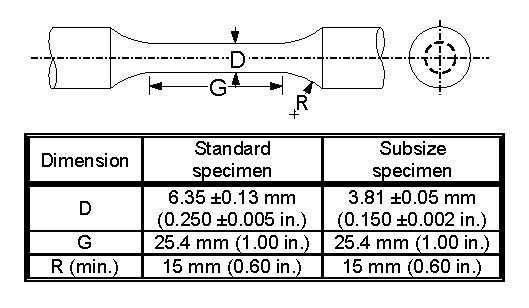
\includegraphics[width=.8\linewidth]{imgs/met/corpo_de_prova}
%       \caption{Corpo de prova utilizado para o teste}
%       \label{fig:corpo_de_prova}
%     \end{subfigure}%
%     \begin{subfigure}{.5\textwidth}
%       \centering
%       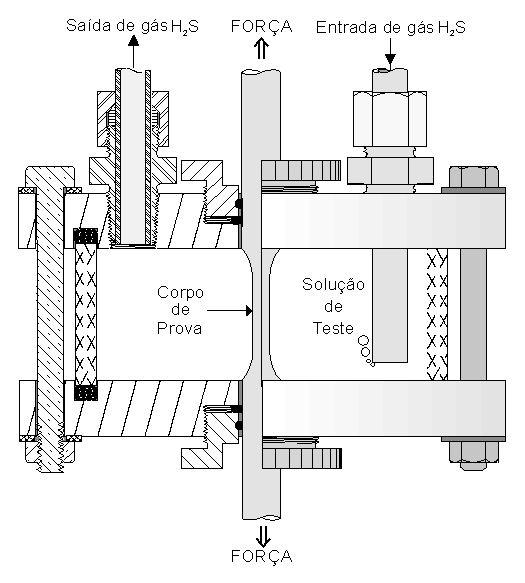
\includegraphics[width=.8\linewidth]{imgs/met/estrutura_de_teste}
%       \caption{Esquemático da câmara para a realização do teste}
%       \label{fig:sfig2}
%     \end{subfigure}
%     \legend{Fonte: NACE Standard TM0177 \cite[p. 7,8]{nace_standart} (Adaptada)}
%     \label{fig:estrutura_de_teste}
%     \end{figure}

% O grande tempo despendido durante o teste e a necessidade de aguardar o resultado para prosseguir para as etapas seguintes de produção resulta em aumento de estoques e altos tempos para o atendimento dos pedidos dos clientes (lead time).

% Diversas características que podem influenciar no resultado do teste foram levantadas e objetiva-se a determinação daquelas com maior significância para a determinação de um modelo capaz de realizar predições do resultado do teste.

% \subsection{Descrição do Conjunto de dados}

% Utilizando-se o conhecimento prévio do processo, uma filtragem inicial dos dados foi realizada, removendo caracteristicas irrelevantes para o processo de modelagem, tais como identificações, lotes e datas. Variáveis que não apresentam nenhuma variação no conjunto de dados também foram removidas. Além disso, por motivos de confidencialidade, o nome das variáveis foram anonimizados. Por fim, os dados passaram pelo processo de normalização descrito anteriormente.

% Após o processamento inicial, o conjunto de dados possui 1064 amostras, com 30 possíveis variáveis de entrada e 3 varíaveis de saída.

% \subsection{Metodologia}

% O objetivo principal nesse estudo é identificar qual o melhor subconjunto de variáveis para descrever o problema. Por isso, o algoritmo proposto foi executado nesse banco de dados e a curva de performance dos subconjuntos levantada. 

% Quatro modelos foram treinados, sendo dois utilizando o conjunto total de variáveis e dois utilizando o melhor subconjunto sugerido pelo método de seleção. Antecipa-se uma melhora de desempenho ao utilizar um conjunto reduzido de variáveis.

% De maneira auxiliar, a correlação linear entre variáveis e a correlação entre saídas e variáveis foi levantada, de maneira a observar se através dessas medidas é possível identificar uma relação com o subconjunto proposto.

\chapter[Resultados e Discussão]{Resultados e Discussão}

\section{Teste do Algoritmo}

O algoritmo foi aplicado a cada um dos bancos de dados indicados na sessão anterior, de maneira a determinar os subconjunto ótimos de variáveis para uso em um modelo de regressão. O resultado obtido determina, a cada iteração, a variável ainda não utilizada que, ao ser acrescentada no modelo, traz a maior redução do erro de validação cruzada (ou o menor aumento). 

A cada iteração "\textit{i}", um subconjunto candidato de \textit{i} variáveis é determinado. O melhor subconjunto é aquele que minimiza o erro LOOCV. É importante reiterar que o algoritmo utiliza uma estratégia de \textit{greedy search} para buscar os subconjuntos e, portanto, a optimalidade global desses subconjuntos não é garantida.

\subsection{Resultados}

\subsubsection{\textit{Communities and Crime}}

No banco de dados \textit{Forest Fires}, o erro de validação cruzada LOOCV mínimo foi observado em um conjunto com apenas 37 das 102 variáveis. A adição de variáveis posteriormente teve pouca influência no erro de validação cruzada, com uma tendência de overfitting na inclusão das últimas variáveis.

O resultado para cada iteração pode ser verificado na figura \ref{fig:stepwise_CommunitiesandCrime_validation}.

\begin{figure}[!htb]
    \centering
    \caption{Seleção de Variáveis \textit{Stepwise: Communities and Crime}.}
    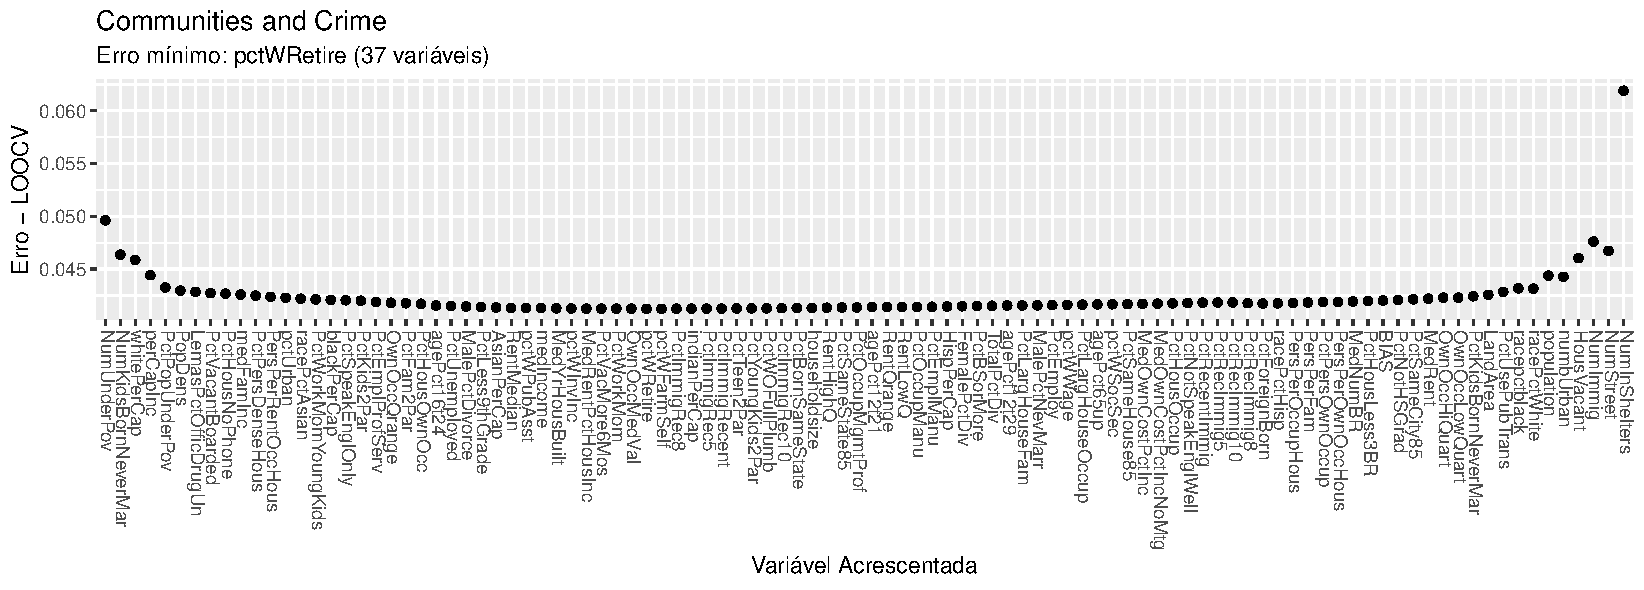
\includegraphics[height=163pt]{imgs/res/CommunitiesandCrime_validation.pdf}
    \legend{Fonte: Própria.}
    \label{fig:stepwise_CommunitiesandCrime_validation}
\end{figure}

\subsubsection{\textit{Forest Fires}}

No banco de dados \textit{Forest Fires}, o erro de validação cruzada LOOCV mínimo foi observado em um conjunto com apenas 4 das 12 variáveis. A adição de variáveis posteriormente resultou em overfitting significativo. 

O resultado para cada iteração pode ser verificado na figura \ref{fig:stepwise_ForestFiresDataset_validation}.

\begin{figure}[!htb]
    \centering
    \caption{Seleção de Variáveis \textit{Stepwise: Forest Fires}.}
    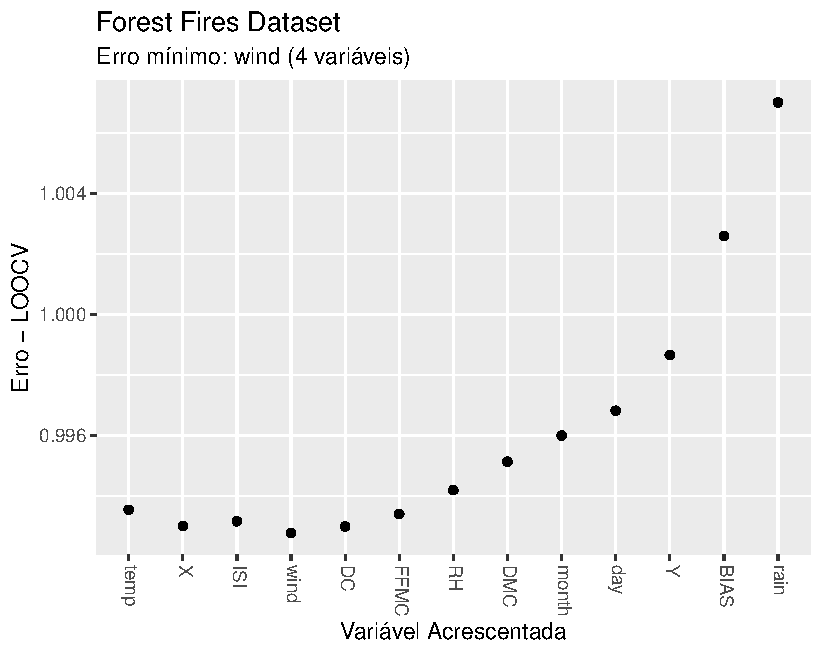
\includegraphics[height=200pt]{imgs/res/ForestFiresDataset_validation.pdf}
    \legend{Fonte: Própria.}
    \label{fig:stepwise_ForestFiresDataset_validation}
\end{figure}

\subsubsection{\textit{USA Housing}}

No banco de dados \textit{USA Housing}, o erro de validação cruzada LOOCV mínimo foi observado em um conjunto com apenas 35 das 80 variáveis. A adição de variáveis posteriormente teve pouca influência no erro de validação cruzada, porém aumentando-o lentamente. 

O resultado para cada iteração pode ser verificado na figura \ref{fig:stepwise_USAHousingDataset_validation}.

\begin{figure}[!htb]
    \centering
    \caption{Seleção de Variáveis \textit{Stepwise: USA Housing}.}
    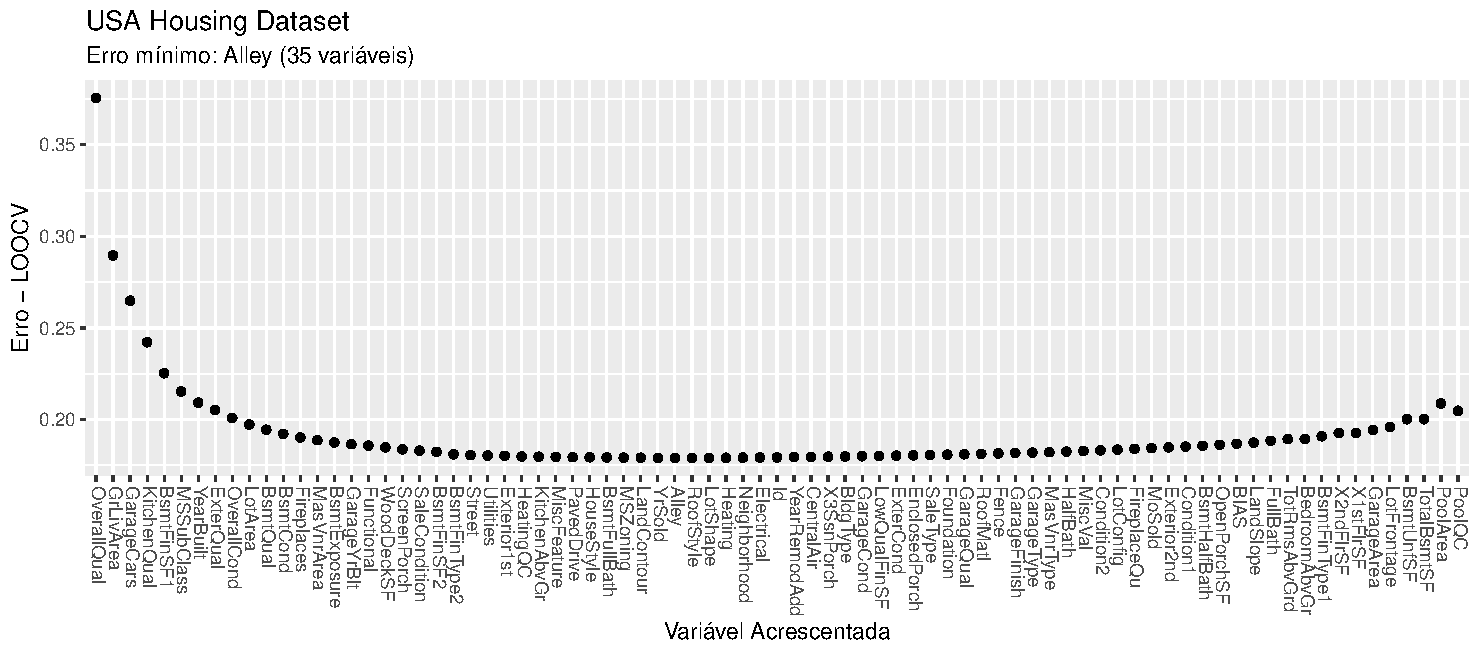
\includegraphics[height=200pt]{imgs/res/USAHousingDataset_validation.pdf}
    \legend{Fonte: Própria.}
    \label{fig:stepwise_USAHousingDataset_validation}
\end{figure}

\subsubsection{\textit{Wisconsin Breast Cancer}}

No banco de dados \textit{Wisconsin Breast Cancer}, o erro de validação cruzada LOOCV mínimo foi observado em um conjunto com apenas 8 das 32 variáveis, e foi identificada também uma tendência significativa ao overfitting quando utilizado um subconjunto candidato de mais de 16 variáveis. 

O resultado para cada iteração pode ser verificado na figura \ref{fig:stepwise_WisconsinBreastCancer}.

\begin{figure}[!htb]
    \centering
    \caption{Seleção de Variáveis \textit{Stepwise: Wisconsin Breast Cancer Dataset}.}
    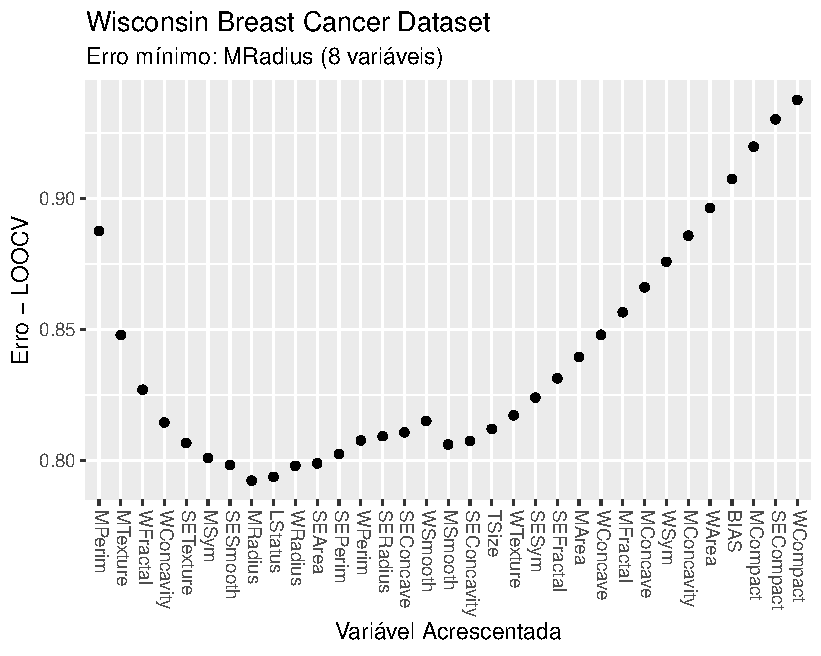
\includegraphics[height=200pt]{imgs/res/WisconsinBreastCancerDataset_validation}
    \legend{Fonte: Própria.}
    \label{fig:stepwise_WisconsinBreastCancer}
\end{figure}


\subsection{Discussão}

Observou-se o decréscimo do erro com o aumento do número de variáveis selecionadas até um ponto de mínimo, a partir do qual a tendência se inverte e o erro passa a aumentar. Tal dinâmica é esperada, uma vez que o aumento do número de parâmetros, na regressão linear, resulta no aumento da complexidade do modelo \cite[p. 224]{statistical_learning}. 

De fato, ao se reduzir a complexidade do modelo através do aumento do parâmetro de regularização ($\lambda$), observa-se a diminuição da tendência ao overfitting, conforme demonstra a figura \ref{fig:lambda_WisconsinBreastCancer}.

\begin{figure}[!htb]
    \centering
    \caption{Efeito do parâmetro de regularização ($\lambda$): \textit{Wisconsin Breast Cancer Dataset}.}
    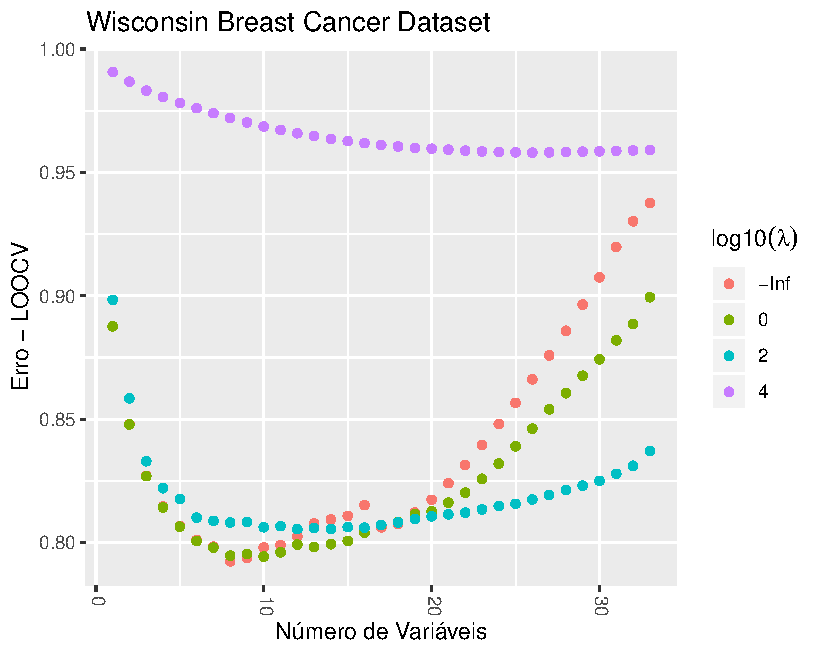
\includegraphics[height=200pt]{imgs/res/WisconsinBreastCancerDataset_lambda}
    \legend{Fonte: Própria.}
    \label{fig:lambda_WisconsinBreastCancer}
\end{figure}

É interessante notar que valores de $\lambda$ reduzidos tiveram pouca ou nenhuma influência nos primeiros subconjuntos ótimos selecionados pelo algoritmo, alterando apenas a seleção na região com tendência ao overfitting. Dessarte, a utilização de um parâmetro de regularização não nulo de pequena magnitude tem pouca influência no conjunto selecionado, enquanto melhora a estabilidade numérica do método, evitando operações com matrizes singulares.

\section{Estudo de Caso: Vallourec - Caracterização de tubos de aço}

\chapter[Conclusão]{Conclusão}

Neste trabalho foi apresentado um método de seleção de variáveis \textit{stepwise} utilizando o erro de validação cruzada \textit{leave-one-out} (LOOCV) em regressores lineares como métrica de performance. O algoritmo proposto faz uso de identidades algébricas conhecidas na literatura para determinar, de maneira incremental, o erro de LOOCV ao se acrescentar uma variável. Dessa maneira, elimina-se a necessidade do ajuste de novos modelos lineares a cada subconjunto de variáveis avaliado.

Os resultados obtidos sugerem a manutenção ou melhora da performance nos bancos de dados considerados ao se utilizar o subconjunto de entradas proposto pelo algoritmo. Além disso, tais subconjuntos são, em todos os casos avaliados, significativamente menores que o total disponível, reduzindo assim o custo computacional e acelerando o treinamento dos modelos.

Diversas técnicas para seleção de variáveis \textit{stepwise} são conhecidas na literatura, porém essas, em geral, utilizam métricas que se baseiam no comportamento assintótico do conjunto de variáveis e presumem diversas restrições em relação ao conjunto de dados e ao modelo a ser desenvolvido. Utilizar o erro de validação cruzada como métrica permite o relaxamento dessas restrições.

A necessidade do armazenamento de uma matriz quadrada da dimensão do tamanho do conjunto amostral é um fator limitante no método proposto. Uma possível solução para tal limitação é a utilização de um número menor de amostras para a seleção de variáveis. Porém a determinação desse número exige ainda um estudo de complexidade amostral (\textit{sample complexity}), aplicando-se teorias tais como complexidade de Rademacher para determinação dos limiares do erro de generalização. Porém tal estudo foge ao escopo deste trabalho.

Por fim, a utilização de regressões lineares é também um fator limitante, uma vez que esses modelos podem falhar em capturar algumas relações não-lineares. Uma possível maneira de minimizar esse problema é utilizar o truque de kernel (\textit{kernel trick})\cite{peaking_phenomenon}, isto é, a aplicar uma função não linear aos dados e utilizar esses dados como entradas no método proposto. Dessa maneira, o algoritmo continua sendo linear em relação às variáveis transformadas, porém se torna não linear em relação aos dados originais.

\bibliography{citations.bib}


%---------------------------------------------------------------------
% INDICE REMISSIVO
%---------------------------------------------------------------------
% \phantompart
% \printindex
%---------------------------------------------------------------------



\end{document}
